Analiza la sucesión que se presenta en la Figura \ref{fig:sucesion_cuadros02}.


\begin{figure}[H]
    \centering
    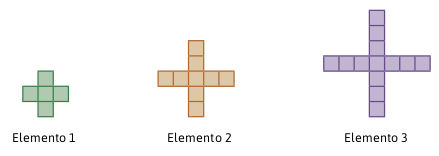
\includegraphics[width=.5\linewidth]{../images/sucesion_cuadros02}
    \caption{}
    \label{fig:sucesion_cuadros02}
\end{figure}
% \begin{multicols}{2}
\begin{parts}
    Completa la Tabla \ref{tab:3.7}
    \vspace{-0.2cm}
    \begin{table}[H]
        \centering
        \caption{}
        \label{tab:3.7}
        \begin{tabular}{r|c|c|c|c|c|c|c|c|}
            \toprule
            \rowcolor{colorrds!80}
            %\cline{2-9}
            {\bfseries\color{white}Posición de la figura} & {\bfseries\color{white}1} & {\bfseries\color{white}2} & {\bfseries\color{white}3} & {\bfseries\color{white}4} & {\bfseries\color{white}5} & {\bfseries\color{white}6} & {\bfseries\color{white}7} & {\bfseries\color{white}8} \\ \hline
            Número de cuadrados                           & \ifprintanswers5\fi       & \ifprintanswers9 \fi      & \ifprintanswers13\fi      & \ifprintanswers17\fi      & \ifprintanswers21\fi      & \ifprintanswers29\fi      & \ifprintanswers37\fi      & \ifprintanswers61\fi      \\ \cline{2-9}
            \bottomrule
        \end{tabular}
    \end{table}

    Escribe una regla de recurrencia para la sucesión.
    \begin{solutionbox}{4em}
        $4n + 1$.
    \end{solutionbox}

    % Reúnete en equipo y comparen sus resultados. ¿Obtuvieron una fórmula igual o equivalente? En caso necesario corrijan y argumenten por qué.

    % \begin{solutionbox}{2cm}
    % \end{solutionbox}
\end{parts}
% \end{multicols}
